\documentclass{article}
\usepackage[utf8]{inputenc}
\usepackage{amsmath}
\usepackage{graphicx}
\usepackage{float}

\graphicspath {}


\title{Networks and Random Processes Assignment 1}
\author{Charlie Pilgrim - 1864704}
\date{October 2018}

\begin{document}

\maketitle


\section{Question 1}



This section considers a Simple Random Walk on ${1,...,L}$ with probabilities $p \in [0,1]$ and $q = 1-p$ to jump right and left respectively. 

Different boundary conditions are considered.

\subsection{Part A}

\subsubsection{Case 1 - Periodic}

Periodic boundary conditions, so $p(0,L) = q$ and $p(L,0) = p$

The transition matrix is:

$P = \begin{bmatrix}
    0 & p & 0 & \dots  & 0 & q \\
    q & 0 & p & \dots  & 0 & 0\\
    0 & q & 0 & \dots  & 0 & 0\\
    \vdots & \vdots & \vdots & \ddots & \vdots \\
    0 & 0 & 0 & \dots & 0 & p \\
    p & 0 & 0 & \dots & q & 0
\end{bmatrix}$

The process is irreducible, i.e. every state can, eventually, reach every other state. And there is a finite state space, so it has 1 unique stationary distribution.

The states can be laid out on a circle, and are symmetrical, so the stationary distribution is where all states have equal probabilities. 

$\pi = (1/L, 1/L,..., 1/L)$

for all $p \in (0,1)$ 

The stationary distribution is reversible only for the case $p=q=\frac{1}{2}$.


\subsubsection{Case 2 - Closed}

Transition matrix:

$P = \begin{bmatrix}
    q & p & 0 & \dots  & 0 & 0 \\
    q & 0 & p & \dots  & 0 & 0\\
    0 & q & 0 & \dots  & 0 & 0\\
    \vdots & \vdots & \vdots & \ddots & \vdots \\
    0 & 0 & 0 & \dots & 0 & p \\
    0 & 0 & 0 & \dots & q & p
\end{bmatrix}$

If $p = 1$, there is an absorbing state at L, and the stationary dsitribution is $\pi = (0,0,...,0,1)$. This stationary distribution is reversible, all terms in the detailed balance equations are zero. This is not irreducible, as the walk can only move from $s_x$ to $s_{x+1}$. 

If $q = 1$, there is an absorbing state at 1, and the stationary dsitribution is $\pi = (1,0,...,0,0)$. This stationary distribution is reversible, all terms in the detailed balance equations are zero. This is not irreducible, as the walk can only move from $s_x$ to $s_{x-1}$. 

If $p = q =\frac{1}{2}$, the process is irreducible, as every state can, eventually, be reached from every other state. There is a finite state space and so there is onle 1 stationary distribution. The sum of all columns equal 1, so there is a constant left eigenvector, and so the stationary distribution is $\pi = (1/L, 1/L,..., 1/L)$. This stationary distribution is reversible.

If $p,q \neq [0,1/2,1]$, then the process is irreducible, and it has a finite state space so there is only 1 stationary distribution. Looing at the detailed balance equations, we can find a recurrence relation of the form:



$\pi_{x-1} p= \pi_x p \text{ over } x = \{2,3,..., L-1\}$


$ \pi_x = \pi_{x-1} \frac{p}{q} $

By induction, this suggests a solution like

$\pi_x = \pi_1 (\frac{p}{q})^{x-1}$

This is a reversible distribution, and so must also be stationary. As the process is ergodic, this is the unique stationary distrubution.

We can check this distribution is staionary for a closed simple random walk with 4 states

 $\begin{bmatrix}
    \pi_1 \\
    \pi_1\frac{p}{q} \\
    \pi_1(\frac{p}{q})^2 \\
    \pi_1(\frac{p}{q})^3 
\end{bmatrix}
\begin{bmatrix}
    q & p & 0 & 0 \\
    q & 0 & p & 0\\
    0 & q & 0 & p\\
    0 & 0 & q & p
\end{bmatrix} = 
\begin{bmatrix}
    \pi_1 \\
    \pi_1\frac{p}{q} \\
    \pi_1(\frac{p}{q})^2 \\
    \pi_1(\frac{p}{q})^3 
\end{bmatrix}$

We also need to normalise the distribution, so the stationary distribution will be

$\pi_x = \dfrac{\pi_1(\frac{p}{q})^{x-1}}{\sum_i^L{\pi_i}}$

\subsection{Part B - Absorbing}

$P = \begin{bmatrix}
    1 & 0 & 0 & \dots  & 0 & 0 \\
    q & 0 & p & \dots  & 0 & 0\\
    0 & q & 0 & \dots  & 0 & 0\\
    \vdots & \vdots & \vdots & \ddots & \vdots \\
    0 & 0 & 0 & \dots & 0 & p \\
    0 & 0 & 0 & \dots & 0 & 1
\end{bmatrix}$

The process is not irreducible, as no other states can be reached from state 1 or state L. 

The (normalised) stationary distributions are

$\pi_1 = [1,0,0,...,0]$

$\pi_2 = [0,0,0,...,1]$

$\pi_3 = [a,0,0,..,0,1-a] \text{ where } a \in [0,1]$



These distributions are reversible, looking at the detailed balance conditions:

$\pi(x)p(x,y) = \pi(y)p(y,x)$ 

All terms for all equations are zero, therefore it is reversible.


\bigskip




The absorption probability in site L is 

$h_k^L = P(X_n = L \text{ for some } n \geq 0|X_0 = k)$


$h_k^L = P(X_n = L \text{ for some } n \geq 0|X_0 = k)$

$h_k^L = P(X_n = L | X_0 = k)$

Considering k+1, k-1, and by law of total probability:

$h_{k}^L = P(X_n = L | X_1 = k+1, X_0 = k) * p + P(X_n = L | X_1 = k-1, X_0 = k) * q $

Using the Markov property:

$h_{k}^L = P(X_n = L | X_1 = k+1) \times p + P(X_n = L | X_1 = k-1) \times q $

\bigskip

$h_{k}^L = h_{k+1}^L \times p + h_{k-1}^L \times q $

And the boundary conditions are:

$h_{1}^L = 0 \text{ and } h_{L}^L = 1$

\bigskip

If $p=q$ then this recursion relation becomes 

$h_{k}^L = \dfrac{h_{k+1}^L + h_{k-1}^L}{2} $

This is linear interpolation between the two surrounding states, so the absorption probability is linear in k. Consdiering the boundary conditions, the solution is:

$h_{k}^L = \frac{k-1}{L-1}$

\bigskip

If $p\neq q$, we can solve the recursion realtion by considering the ansatz:


$h_{k}^L = \lambda^k $

$\lambda = p \lambda^2 + q$

This has roots:

$\lambda_1 = 1 \text{ and } \lambda_2 = q/p$



The general solution is of the form:

$h_k^L = a\lambda_1 + b\lambda_2$ 

$h_k^L = a + b(\frac{q}{p})^k$ 


Looking at the boundary conditions:

$h_1^L = 0 = a + b(\frac{q}{p})$

$h_L^L = 1 = a + b(\frac{q}{p})^L$

Subtracting the first equation from the second equation, and solving for b:

$b = \dfrac{1}{(\frac{q}{p})^{L}-\frac{q}{p}})$

$a = \dfrac{-1}{(\frac{q}{p})^{L-1}-1}$


\subsection{Part C - simulations}

A simple random walk with L=10 and closed boundary conditions was simulated 500 times, with a $p=0.6$ and starting at x=1 at t=0.

\begin{figure}[H]
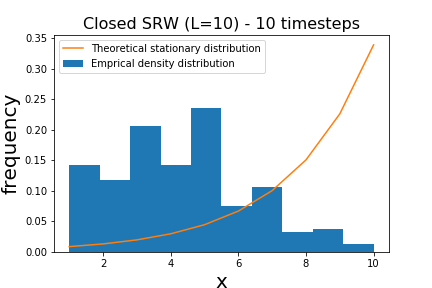
\includegraphics[scale=1]{10_steps_a.png} 
\small{Figure 1. The frequency distribution over 500 different realisations after 10 timesteps.}
\end{figure}

After 10 time steps (Figure 1), the state of the process is still heavily influenced by the starting condition of x(0) = 1. 

\begin{figure}[H]
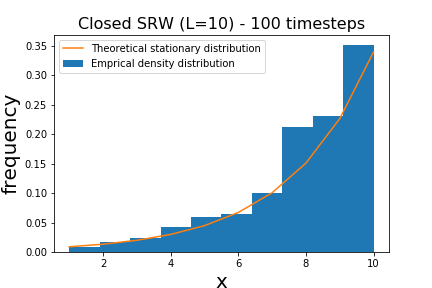
\includegraphics[scale=1]{100_steps_a.png} 
\small{Figure 2. The frequency distribution over 500 different realisations after 100 timesteps.}
\end{figure}

After 100 time steps (Figure 2), the empirical distribution is similar to the theoretical stationary distribution. Ergodic processes tend towards the stationary distribution after a large number of time steps.


\begin{figure}[H]
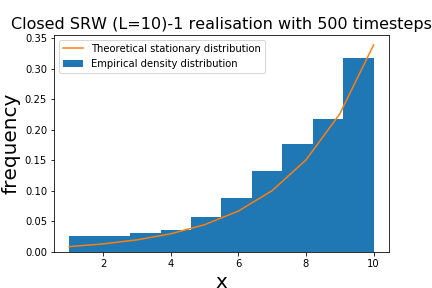
\includegraphics[scale=1]{500_steps_a.png} 
\small{Figure 3. The frequency distribution of states over 500 timesteps of 1 realisation of the simulated simple random walk.}
\end{figure}

After 500 time steps of 1 realisation(Figure 3), the empirical distribution is similar to the theoretical stationary distribution. This is jsut 1 realisation, so there is a lot of stochasticity in the specific distribution generated. This is a reasonably good representative example.



\section{Question 2}

$X_1, X_2, ... $ is a sequence of independent, identically distributed random variables (iirdvs) with 

$X_i \sim N(\mu, \sigma^2)$ 

$\mu \in {R}$ and $\sigma^2 > 0$

Discrete time random walk on state space ${R}$

$(Y_n : n \geq 0)$ with $Y_{n+1} = Y_n + X_{n+1}$ and $Y_0 = 0$


\subsection{Part A}

The weak law of large numbers for $Y_n$:

$\frac{1}{n}Y_n = \frac{1}{n}\sum\limits_{k=1}^n X_k -> \mu \text{ as } n -> \infty$

The expected value of $\frac{Y_n}{n}$ will converge to $\mu$ with large n.

\bigskip
The central limit theorem for $Y_n$:

$\dfrac{Y_n - n\mu}{\sigma n^\frac{1}{2}} = \dfrac{1}{\sigma n^\frac{1}{2}}\sum\limits_{k=1}^n (X_k - \mu) -> \xi \text{ as } n -> \infty$

where $\xi \sim N(0,1)$

\subsection{Part B - distribution of $Y_n$}

$Y_n \sim N(n\mu, n\sigma^2)$

$Y_n$ is approxiamtely normally distributed with mean equal to $n\mu$, where $\mu$ is the mean of the random variable $X$, and with variance $n\sigma^2$, where $\sigma^2$ is the variance of the random variable $X$. 

\subsection{Part C}

$Z_n$ has a recurive relationship given by

$Z_{n+1} = exp(Y_n + X_{n+1})$

$Z_{n+1} = Z_n exp(X_{n+1})$

\subsubsection{Derivation of pdf}

$Y$ is distributed normally, and

$Y = ln(Z)$

\bigskip

Consider the cumulative distribution function:


$F_z(z) = P(Z \leq z) = P(Y \leq ln(z)) = F_y(ln(z)) = \Phi(\dfrac{ln(z) - n\mu}{\sigma \sqrt{n}})$

$f_z(z) = \frac{d}{dz}F_z(z)$

by the chain rule, this gives

$f_z(z) = \dfrac{1}{z} \dfrac{1}{\sigma_y \sqrt{2\pi}}exp(\dfrac{-(ln(z)-\mu_y)^2}{2\sigma_y^2})$

Or, in terms of the standard deviationa nd mean of x

$f_z(z) = \dfrac{1}{z\sigma_x \sqrt{2n\pi}}exp(\dfrac{-(ln(z)-n\mu_x)^2}{2n\sigma_x^2})$

$Z_0$ is fixed by the initial conditions as $Z_0=1$. So the log-normal distribution given above applies for $n \geq 1$.

\bigskip

From wikipedia: 

$E(Z_n) = exp(n\mu + \frac{n\sigma^2}{2})$

$Var(Z_n) = exp(2n \mu + n\sigma^2)(exp(n\sigma^2)-1)$

$Med(Z_n) = exp(n\mu)$

Where $\mu$ and $\sigma^2$ are the mean and variance of X.

\subsection{Part D}
$Z_n$ was simulated 500 times over 100 timesteps with $\mu_x=0$ and $\sigma_x=0.2$. 

\subsubsection{Empirical Average}
Figure shows the empirical average of $Z_n$ as a function of time, $n$. The error bars show the emprical standard deviation at each point.

INSERT EMPRICAL AVERAGE FIGURE

\subsubsection{Boxplots}
Figure shows boxplots of the empirical average and range at $n=10$ and $n=100$. 

INSERT BOXPLOTS FIGURES

\subsubsection{Emprical PDF and theoretical PDF}
Figure shows a kernel desinity estimation of the probability density funtion, with the theoretical prediction, for timesteps $n=10$ and $n=100$. 

INSERT KDE FIGURES

\subsubsection{Ergodic Average}
Figure shows the ergodic average for 4 different single realisations plotted over 100 timesteps. 

\subsection{Part E}

We want 

$E(Z_n) = 1 \text{ for all } n\geq0$

$E(Z_n) = exp(n\mu + \frac{n\sigma^2}{2}) = 1$

$\mu + \frac{\sigma^2}{2} = 0$

$\mu = - \frac{\sigma^2}{2}$

$\mu = -\frac{1}{50}$

Figure shows the emprical tail of the data compared to the theoretical survival function, defined as 1 minus the cumulative distribution function.




\section{Question 3}

\subsection{Part a}


Each individuum can have the starting type of any other individuum. If we consider a vector that contains all of the unique starting states, $b_0 = [X_0(1), X_0(2), . . . , X_0(L)]$, then each individuum can be any element in that vector. This gives a state space of size $L^2$. In mathematical notation:


$X(i) \in X_0(j) \ \text{ where } \ i,j \in \{1,2,...,L\}$ 


The process is not irreducible, as once a type goes extinct it stays extinct, and so not every state can be reached from every other state.

The stationary distributions are where all individuals are of one type i.e. all $X(i)$ are equal to the same one of the initial types $X_0(j)$. In mathematical notation:

$ \forall X(i) : X(i) = X_0(j) \text{ where } j \in \{1,2,..,L\}$  

\subsection{Part b}

\subsubsection{State space}

The future state of the process depends only on the current state at each time step, so yes it is Markov. 

The state space is 

$N_i \in {0,1,...,L} \text{ and } \sum\limits_i^LN_i = L$ 

For each type, there can be an integer number of individuals of that type between 0 and L. Their is the constraining condition that the total indiivduals is always L. 

\subsubsection{Transition Probabilities}

Let $N_t(j)$ be the number of individuals of a particular species, $j$ in a generation, and L individuals in total. For indiviudal of the next generation, the probability of being of this particular species is equal to the proportion of individuals of that type in the parent generation. 

$p(X_{t+1}(i) = j) = N_t(j)/L$

So the transition probabilites for $N_t+1$ are given by a binomial distribution:

$p(N_{t+1}(j) = k) = {L \choose k}(\frac{N_t(j)}{L})^k(1-\frac{N_t(j)}{L})^{L-k}$

The process is not irreducible, if the number of indiviudals of the given species reaches zero, then it is extinct and can never grow again above zero. If the number of individuals reaches L, then this species is the only species left and will always remain so. 

\subsubsection{Stationary Distributions}

If we define a distribution vector as

$\pi = [N_t(0), N_t(1),...,N_t(L)]$

Then there are stationary distributions on the absorbing states

$\pi_1 = [1, 0,...,0,0]$

$\pi_2 = [0, 0,...,0,1]$

and any normalised linear combination of these states, so

$\pi_0 = [a, 0,...,0,1-a] \text{ where } a \in [0,1]$ 

With the initial condition $N_0 = 1$, there is one individual of this type in the population. By symmetry, the probability of this species taking over has to be equal to $1/L$. So the limiting distribution as $t -> \infty$ is

$\pi_{\infty} = [1-\frac{1}{L},0,...,0,\frac{1}{L}]$



The process is not irreducible, as once a state has $N_i = 0$ for any i, i.e. a type goes extinct, the state space where $N_i >0$ is no longer accessible.

The stationary distributions are where 

$N_i = \delta_{i,j}L \text{ where } j \in \{1,L\}$

Q. Limiting distribution?










\end{document}





